\section{Intro}
\label{sec:intro}
Implementer et AVL og Splay datastruktur. Implementeringen skal indeholde:
\begin{itemize}
\item Insert(): Til at indsætte en ny værdi.
\item Contains(): Til tjek om værdien allerede findes i træet.
\end{itemize}
Det er ikke nødvendigt med en remove-funktion, men det er i orden at lave den funktion alligevel.\\
Strukturen skal testes på forskellige størrelser af datasæt, hvorved tiden undersøges i forhold til datastørrelsen. Forsøget skal foretages med tre forskellige typer af datasæt:
\begin{itemize}
\item [Inc:] Værdi som monotomt øges.
\item [Dec:] Værdi som monotomt sænkes.
\item [Ran:] Værdi som vælges vilkårligt.
\end{itemize}

\section{Implementering}
\label{sec:implementation}
Hele implementeringen er bestående af følgende moduler:
\begin{itemize}
\item main.cpp. Kode findes i appedix \ref{app:main}.
\item AvlTree.h og AvlTree.cpp. Kode findes i appedix \ref{app:avl}.
\item SplayTree.h og SplayTree.cpp. Kode findes i appedix \ref{app:splay}.
\item clock\_timer.h og clock\_timer.cpp. Er ikke vedlagt denne raport.
\end{itemize}

Til implementering af AVL og Splay datastruktur er henholdvis følgende links brugt til inspiration/implementering: \url{http://www.sanfoundry.com/cpp-program-implement-avl-trees/} og \url{http://www.sanfoundry.com/cpp-program-implement-splay-tree/}.\\
Hovedprogrammet er lavet således at før programmet kommer ind i main(), implementeres en funktion som generer de tre datalister med ønsket antal elementer, der senere skal bruges af de to implementeringer. Det er ligeledes den første function som der køres i main(). Herefter laves et objekt til hver implementeret klasse. Så udskrives information, der beskriver hvilke funktioner programmet indeholder. Hvorefter det er muligt at vælge hvilken funktionalitet der skal udføres. Funktionaliteten udføres og programmet slutter.

\section{Data/plots for implementeringerne}
Som nævnt i ovenstående afsnit \ref{sec:implementation}, er de to implementationer kørt for de tre forskellige datasæt Inc, Dec og Ran. Undersøgelserne er kun kørt én gang for hver datasæt for et givet N. Hvis forsøgene fortages flere gange for samme datastørrelse gives en mere korrekt billede af de to implementeringer.\\
Indsætning af dataværdier og tjek på forskellige dataværdier er beskrevet i de to næste afsnit, hhv. afsnit \ref{subsec:ind} og afsnit \ref{subsec:find}. Implementeringstiderne samt søgetiderne opsummeres i afsnit \ref{subsec:op}.

\subsection{Indsætning af de tre datasæts}
\label{subsec:ind}
Tabel \ref{tb:balance} viser de seks implementeringstider angivet i [ms] og implementeringstiderne er plottet i figur \ref{fig:balance}.

\begin{figure}[th!]
\centering
\resizebox{\linewidth}{!}{%
\begin{tabular}{l|c|c|c|c|c|c|c|c|c|c|c|c|c|c}
N/datasæt&5&10&20&40&80&160&320&640&1280&2560&5120&10240&20480&\\\hline 
AVL Inc&3,064&3,067&3,147&3,562&3,166&4,96&6,045&7,911&23,441&74,205&284,033&1123,63&4621,95&[ms]\\
AVL Dec&0,03&0,04&0,045&0,108&0,252&1,359&4,795&13,792&54,942&210,587&853,775&3501,78&13801,2&[ms]\\
AVL Ran&3,074&3,098&3,186&3,707&3,545&7,233	&11,779&29,963&115,763&457,994&1894,21&7886,95&32435&[ms]\\
Splay Inc&0,04&0,059&0,054&0,128&0,266&1,403&4,835&13,851&55,071&210,811&854,414&3502,61&13802,7&[ms]\\
Splay Dec&3,08&3,097&3,191&3,714&3,55&7,247&11,789&29,975&115,787&458,051&1894,33&7887,11&32435,3&[ms]\\
Splay Ran&0,045&0,067&0,06&0,137&0,278&1,431&4,881&13,914&55,181&211,017&855,104&3503,45&13804,4&[ms]
\end{tabular}}
\captionsetup{type=table}
\caption{Implementeringstider for de seks datalister som funktion af datasætstørrelsen N.}
\label{tb:balance}
\end{figure}
\begin{figure}[th!]
\centering
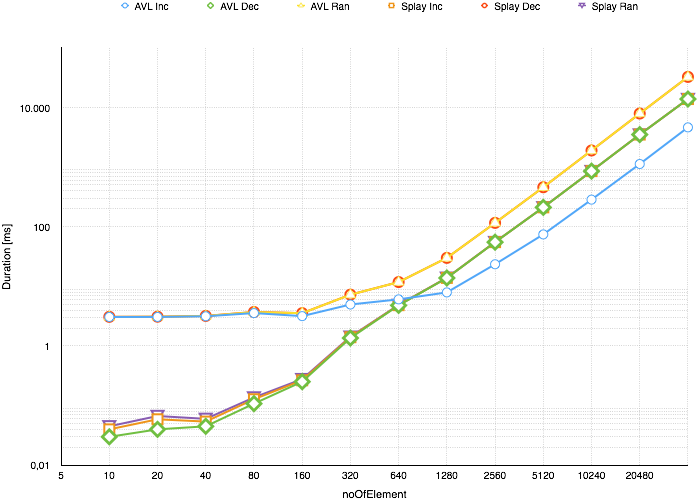
\includegraphics[width=.8\textwidth]{./graphics/balance}
\caption{Logaritmisk plot af implementeringstider for datasætstørrelserne N.}
\label{fig:balance}
\end{figure}

For at kunne sammenligne de to datastrukturer er \(\Delta\)-værdien mellem AVL og Splay beregnet. Hvis \(\Delta\)-værdien er positiv er Splay strukturen hurtigst og omvendt. \(\Delta\)-værdierne er angivet I tabel \ref{tb:delta_balance}. \\
For datasættet Inc er Splay strukturen hurtigst indtil en datastørrelse på 640 elementer. Herefter overtager AVL strukturen.\\
For Dec datasættet ses der at AVL strukturen har den hurtigste implementeringstid for de afprøvede datasæt med N elementer. \\
For Ran datasættet er implementeringstiderne generelt hurtigere ved Splay strukturen.

\begin{figure}[th!]
\centering
\resizebox{\linewidth}{!}{
\begin{tabular}{l|c|c|c|c|c|c|c|c|c|c|c|c|c|c}
N/datasæt&5&10&20&40&80&160&320&640&1280&2560&5120&10240&20480&\\\hline 
\(\Delta\)Inc&3,024&3,008&3,093&	3,434&2,9&3,557&1,21&-5,94&-31,63&-136,606&-570,381&-2378,98&-9180,75&[ms]\\
\(\Delta\)Dec&-3,05&-3,057&-3,146&-3,606&-3,298&-5,888&-6,994&-16,183&-60,845&-247,464&-1040,555&-4385,33&-18634,1&[ms]\\
\(\Delta\)Ran&3,029&3,031&3,126&3,57&3,267&5,802&6,898&16,049&60,582&246,977&1039,106&4383,5&18630,6&[ms]
\end{tabular}}
\captionsetup{type=table}
\caption{\(\Delta\)-værdien er angivet som differencen mellem implementeringstiden for AVL og Splay i [ms].}
\label{tb:delta_balance}
\end{figure}
\begin{figure}[th!]
\centering
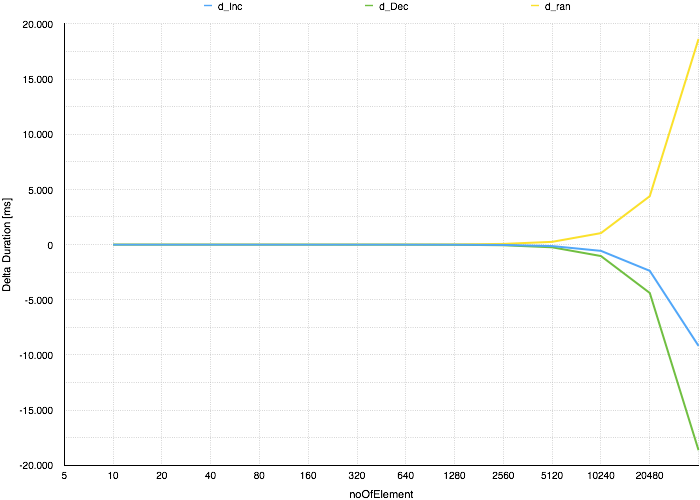
\includegraphics[width=.8\textwidth]{./graphics/delta_balance}
\caption{Plot af \(\Delta\)-værdien for de tre datasæt for en given datastørrelse N.}
\label{fig:delta_balance}
\end{figure}

Figur \ref{fig:delta_balance} viser \(\Delta\)-værdierne mellem AVL og Splay implementeringerne for en given datastørrelse. For en positiv difference er Splay implementeringen hurtigst og ligeledes med en negativ difference er AVL implementeringen hurtigst.
	
\subsection{Find vilkårlig værdi i datasæt}
\label{subsec:find}
I tabel \ref{tb:find_key} ses søgetiden for en vilkårlig værdi. Værdien er forsøgt fundet i en AVL og Splay struktur med et vilkårlig generet datasæt med N antal elementer. Tabellen angiver også den søgte værdi og ligeledes en \(\Delta\)-søgetid for de to strukturer. Figur \ref{fig:find_key} indeholder et plot af søgetiderne.

\begin{figure}[th!]
\centering
\resizebox{\linewidth}{!}{
\begin{tabular}{l|c|c|c|c|c|c|c|c|c|c|c|c|c|c}
N/datasæt&5&10&20&40&80&160&320&640&1280&2560&5120&10240&20480&\\\hline 
AVL&	 3,464&3,158&3,014&4,114&3,061&3,467&4,43&7,839&22,422&79,205&339,533&1540,28&6989,17&[ms]\\
Splay&0,011&0,013&0,014&0,014&0,028&0,025&0,043&0,075&0,131&0,235&0,565&0,91&1,736&[ms]\\
\(\Delta\)&3,45&3&3,145	3&4,1&3,033&3,442&4,387&7,764&22,291&78,97&338,968&1539,37&6987,434&[ms]\\\hline
Ran number&4&2&18&20&62&137&29&364&449&2510&2400&3960&8303&
\end{tabular}}
\captionsetup{type=table}
\caption{Søgetider for AVL og Splay samt differencen i mellem angivet som \(\Delta\) for en given datastørrelse. Og ligeledes vises det vilkårlige nummer for den given datastørrelse.}
\label{tb:find_key}
\end{figure}

\begin{figure}[th!]
\centering
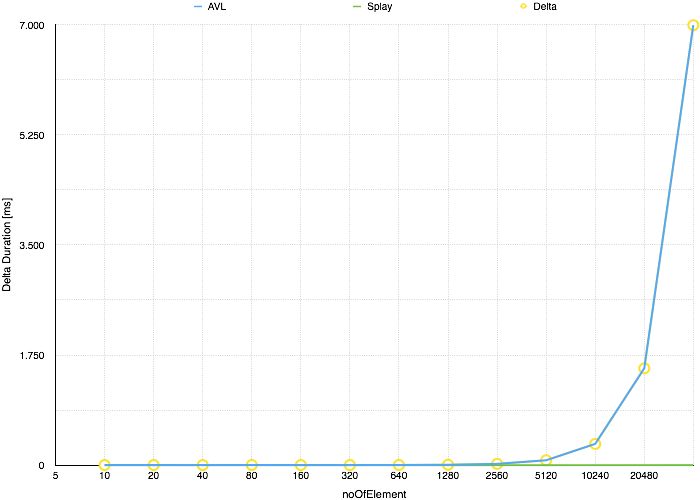
\includegraphics[width=.8\textwidth]{./graphics/findkey}
\caption{Plot af søgetiderne efter en vilkårlig værdi i datasæt for AVL, Splay samt differencen \(\Delta\) for et givet datasæt med given datastørrelse N.}
\label{fig:find_key}
\end{figure}
I tabel \ref{tb:find_key} er det tydeligt at se at Splay implementeringen er langt hurtigere til at finde den vilkårlige værdi i et givet data sæt. Dette underbygges af plottet i figur \ref{fig:find_key}.


\subsection{Opsummering}
\label{subsec:op}
AVL strukturen:
\begin{itemize}
\item Er hurtigst for Dec datasættet.
\item Er hurtigst for Inc datasættet efter dets datastørrelse er over 320 elementer.
\end{itemize}
Splay strukturen:
\begin{itemize}
\item Er hurtigst for Inc datasættet for en datastørrelse på 5-320 dataelementer.
\item Er hurtigst for Ran datasættet.
\item Er hurtigst til at finde en vilkårlig værdi for et Ran datasæt. 
\end{itemize}
Idet AVL og Splay strukturerne har forskellige karakteristika er det essentielt at kende applikationen for at kunne benytte den mest optimale datastruktur.  


\section{Konsol output}
Figur \ref{fig:console} viser et screenshot fra den bruge editor xCode. I programmet genereres de tre datasæt på 20 elementer hver og bruges i case option 4 til returnering af tiderne det tager for AVL og Splay strukturerne at indsætte de tre datasæt.
\begin{figure}[th!]
\centering
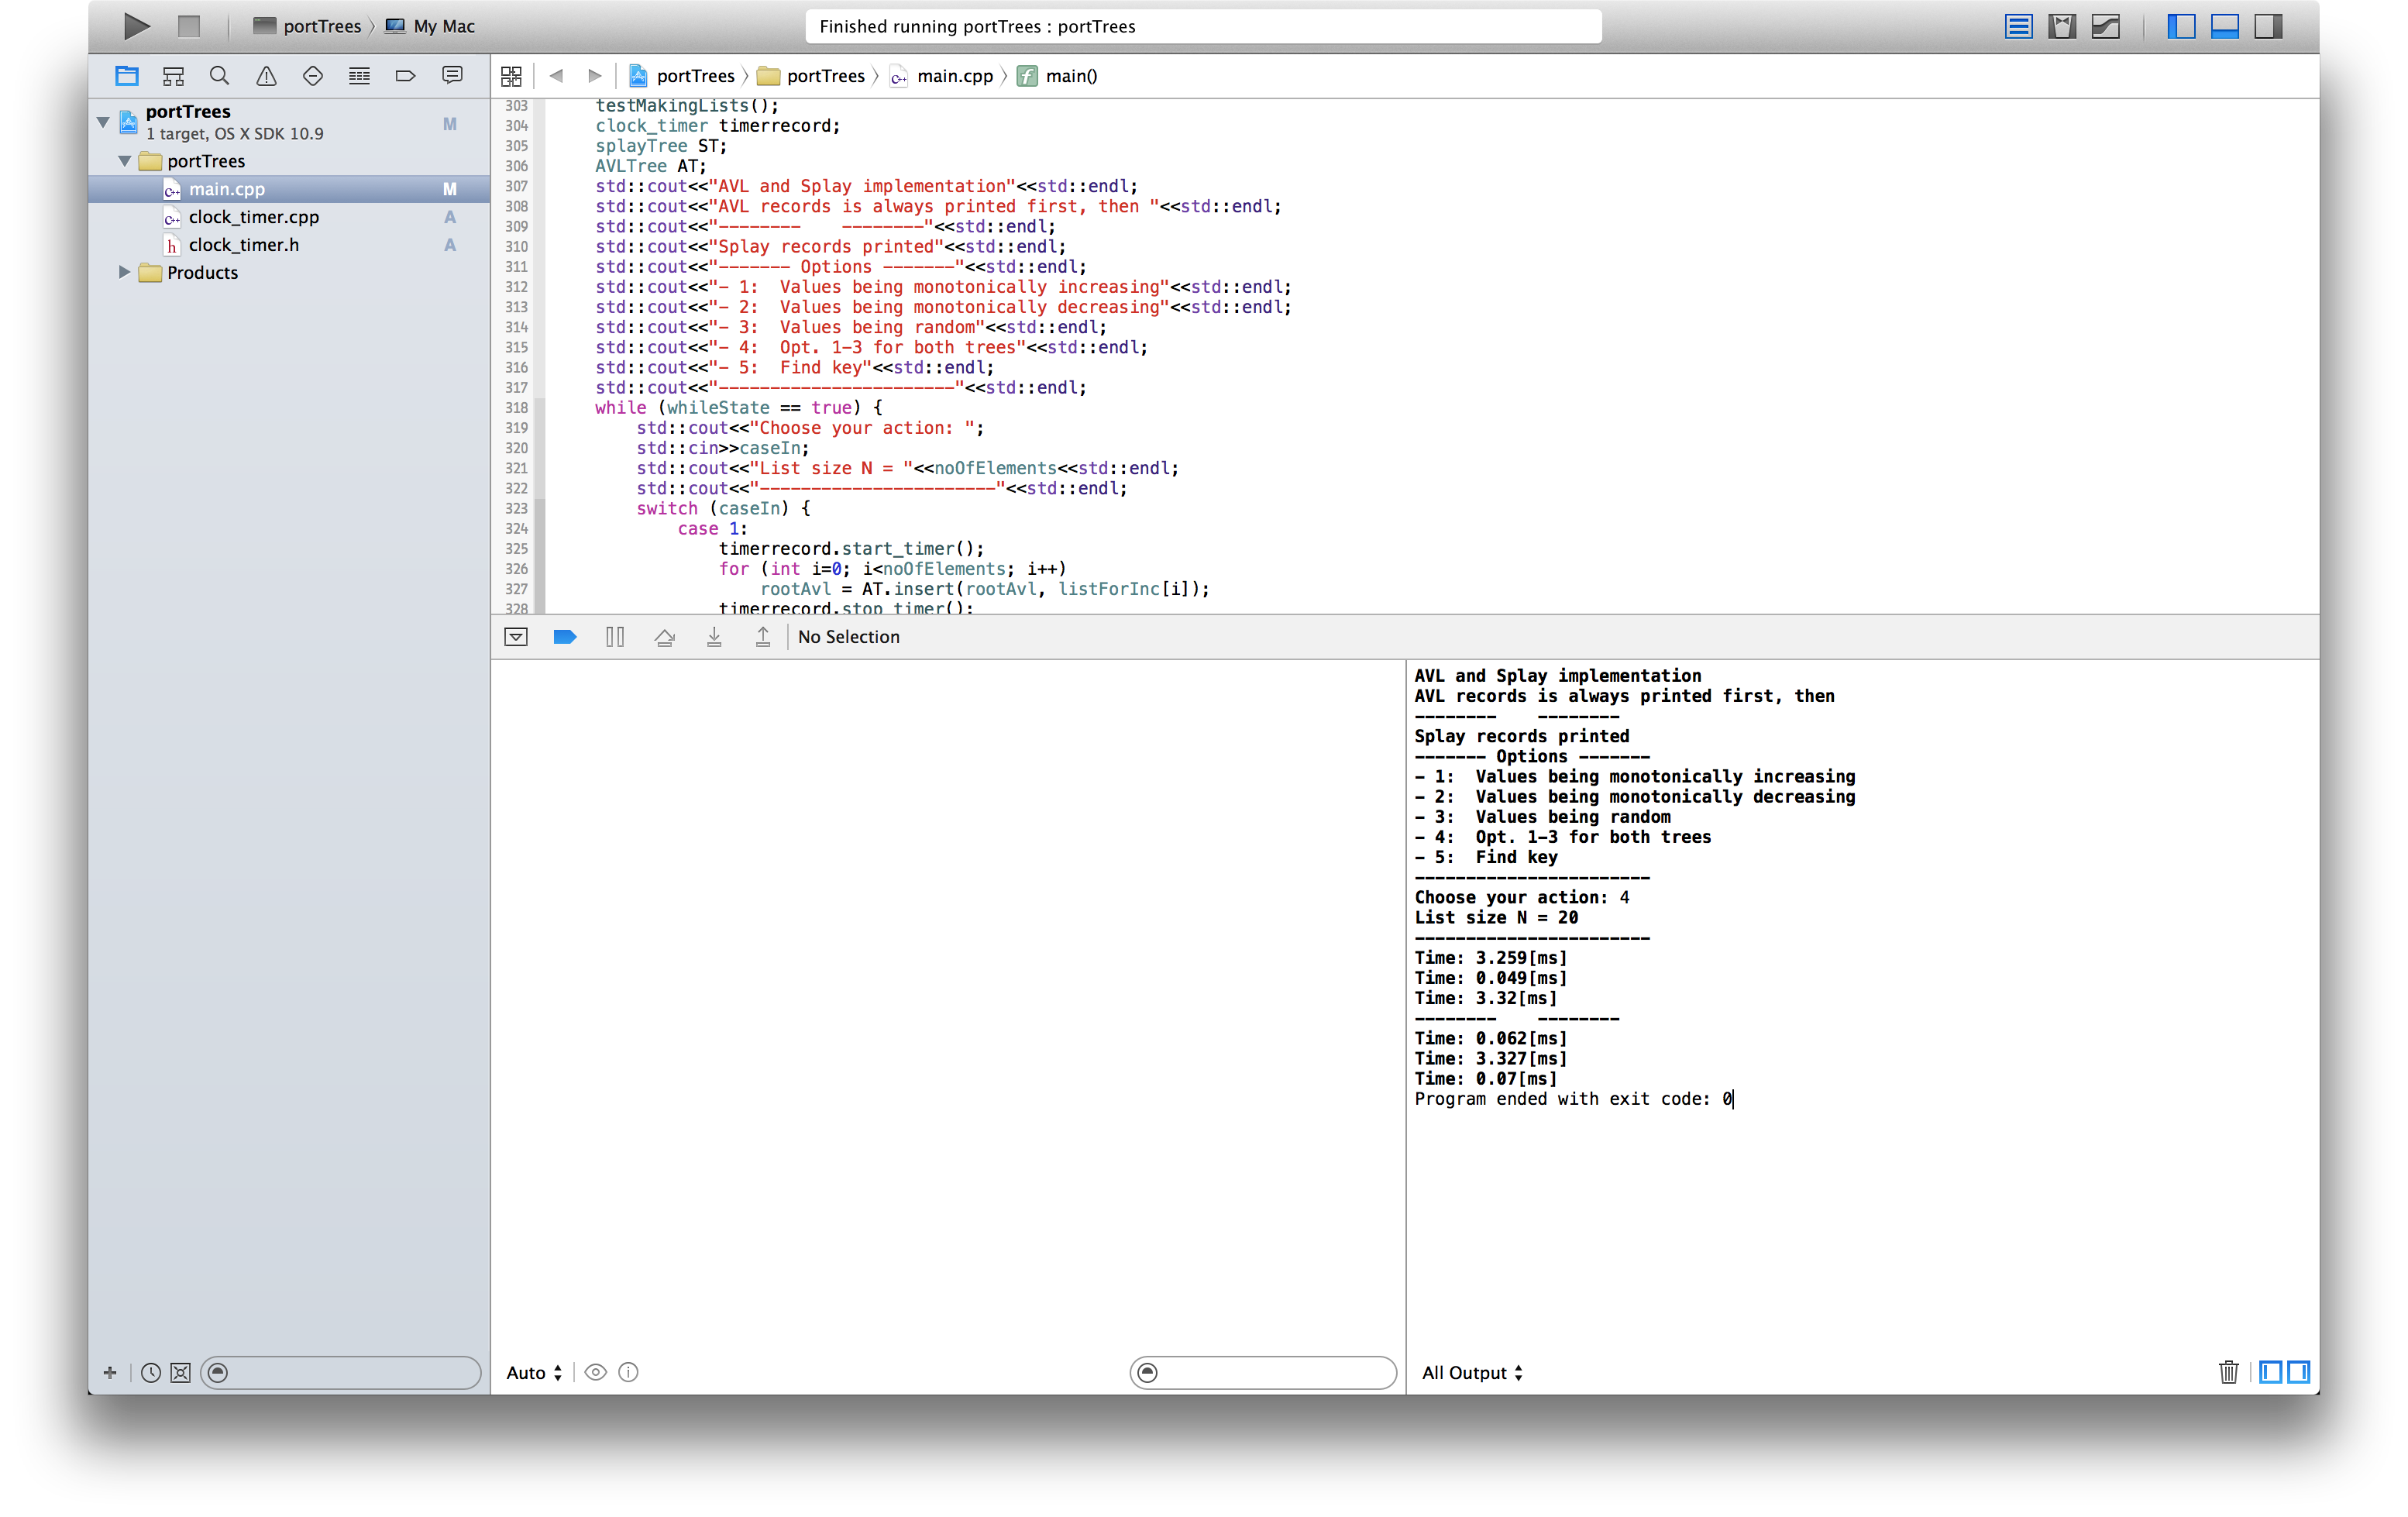
\includegraphics[width=0.75\textwidth]{./graphics/console}
\caption{Konsol output med implementeringstid for de tre datasæt af 20 elementer: case action 4.}
\label{fig:console}
\end{figure}